\documentclass{article}
\usepackage[margin=1in]{geometry}

\usepackage{amsmath,graphicx}
\usepackage{physics}

\title{TDSE Code - User Guide, Best Practices, and Developers Notes}
\author{J. Venzke}

\begin{document}
\maketitle

\tableofcontents
\newpage

\section{Introduction} % (fold)
\label{sec:introduction}
\subsection{Code Overview} % (fold)
\label{sub:code_overview}
The TDSE code discussed here was initially developed by Joel Venzke while working on his Ph.D. in the Ultrafast Theory Group in JILA. Cory Goldsmith and other group members have also contributed to this code in various forms. It solves the Time Dependent Sch\"{o}dinger Equation (TDSE) for various targets in a laser field for a single active electron. It has support for two or more active electrons, but the computational power of modern super computers limits the calculation that are possible to 2 electrons in 2 spacial dimensions. For single active electrons, I have developed a cylindrical 2D code for linear polarized light. The cylindrical code can support aligned molecular targets for SAE potentials. For atomic targets, utilize the spherical code which is orders of magnitude more efficient and supports arbitrary laser polarizations. All other calculations requirer use of the Cartesian grid code. There is an RBF implementation, but due to issues with the eigenvalues behaving poorly time propagation is not currently working. Future work will look to push towards a 2 electron full 6D code, and extending the code to different coordinate systems/basis methods.

This code has support for real space propagation of the TDSE using finite differences for spacial derivatives and Crank-Nicolson for time propagation. The codes has been shown to scale out to 3,000+ processors. It can also simulate interesting physics on a laptop if you have a few hours of free time. The main drive for developing this code is to allow for many types of laser interactions to be studies in a single code base.
% subsection code_overview (end)

\subsection{Problems of interest} % (fold)
\label{sub:problems_of_interest}
At the attosecond ($10^{-18} seconds$) time scale, molecular motion is frozen, and electron dynamics dominate all processes. In order to study how electrons interact with attosecond laser pulses, we solve the Time-Dependent Sch\"{o}dinger Equation (TDSE). This can be done relatively easily for 1 electron with linear polarized light, however, circular polarization and multi-electron effects make the calculations more computationally interesting. Gaining a deeper understanding the behavior of electrons induced by intense ultrashort laser pulses is the reason this code is being developed.
% subsection problems_of_interest (end)


\subsection{Development Goals} % (fold)
\label{sub:development_goals}
This code is being designed with large scale numeric simulation in mind. By limiting the code by the size of a supercomputer rather than the clock speed of a fast desktop, physics that would be otherwise out of reach can be studies provided one obtains the required computing resources. That being said, for small scale simulation, there are more efficient codes that take advantage of the shared memory architectures. However, those codes will reach limitations due to hardware which is where a large scale code like this starts to shine. For that reason, MPI is used for parallelization so that we can utilize HPC systems with distributed memory.

Since this code is for physics, we want the users to be able to focus on physics rather than the computer science back end. As a result, the pipe dream is to have all simulations only require an input file with no need to write code. It maybe necessary to learn python for custom data visualizations, but many of the visualizations needed to analysis the results are included with the repo. You may also need to implement small c++ changes if you wish to simulate targets that do not fit the current layout or various other unsupported tasks, though I hope to make this code relatively general.

It would also be nice that when the simulation is complete, the code produces enough plots to make sure that the simulation worked and a basic overview of the interesting physics the simulation contains. For this reason, all visualization is done in a batch mode and images are saved in a ``figs'' directory. You can use the Observables.h5 (Sec.~\ref{sub:observables_h5}) file to copy small datasets back to your local machine to further analyze the data.

Finally, I want this code be useful in future iterations. Therefor I used GitHub for version control. I have also been working on providing documentation to make the code more transparent and easier to use.
% subsection development_goals (end)

\subsection{Key Features} % (fold)
\label{sub:key_features}
TODO
% subsection key_features (end)

\subsection{Recommended Programing Background} % (fold)
\label{sub:recommended_programing_background}
It is recommended you are familiar with python including the numpy, matplotlib, and h5py modules. This will allow you to make changes to the analysis software and analyze the results of the code beyond what already exists. It is also recommended you are familiar with the command prompt (terminal). Useful knowledge includes general bash commands such as cd, mkdir, sed, grep, chmod, and how to execute a binary file. There are other commands such as mpiexec, h5ls, and h5dump that are useful to know, but will be talked about when needed in this documentation. You should also become familiar with any schedulers you may need to use on the various clusters and super computers you plan to use. Most of the script associated with this package have been designed for SLURM with some being designed for Torque (PBS).

If you need to update the main code, you will need knowledge of C++. Most updates at this point are standard C++ code, however, the PETSc and SLEPc libraries are used for any matrix vector operations, the IO is preformed through the HDF5 library, MPI calls are often done with Boost MPI, and GSL has been used for some special functions.
% subsection recommended_programing_background (end)
% section introduction (end)

\section{Installation} % (fold)
\label{sec:installation}
Compiling the TDSE library itself is easy. However, some of the dependencies are tricky to get installed. Here is a short overview with some tips and tricks to help you out. Please read the  If you run into issues, shoot me an email.

The steps required to install this code are as follows. More detailed directions are in the following subsections.
\begin{enumerate}
  \item Choose the compiler you plan on using
  \item Check module system/package manager for dependencies
  \item Install HDF5 (special version required, C++ and MPI)
  \item Install PETSC (link HDF5)
  \item Install SLEPC
  \item Install TDSE library
  \item Update your bashrc file
\end{enumerate}

% subsection overview (end)

\subsection{Compilers} % (fold)
\label{sub:compilers}
This code has been installed with gcc and intel compilers with c++11 or better support. Portland group compilers have not been tested, but should work. If you are using a Mac, install gcc with the homebrew package manager (https://brew.sh) instead of using clang as you will need a fortran compiler for PETSC.
% subsection compilers (end)

\subsection{Dependencies} % (fold)
\label{sub:dependencies}
Before beginning the install process, make sure the following software is installed on your computer. Make sure they are compiled with the compiler you intend on using to compile the TDSE library. You should find them on the module system at most HPC centers and many local clusters. Here is the list of packages to look for:
\begin{itemize}
  \item boost  
  \item boost-mpi 
  \item cmake
  \item gsl   
  \item open-mpi (or equivalent)
  \item zlib (can be installed by HDF5)
\end{itemize}
If one or more of these packages are not installed, you will need to do so manually. For Mac users, I recommend using homebrew (https://brew.sh) as your package manager and start by installing gcc followed by the rest of the packages. I have not had to install these packages on any other system, so if you need to, talk to a system admin or try your hand at installing them off their website.
% subsection dependencies (end)

\subsection{HDF5} % (fold)
\label{sub:hdf5}
\begin{enumerate}
  \item Download and untar HDF5 source (https://www.hdfgroup.org)
  \item Make the directory you wish to install HDF5 in
  \item cd to the directory you just make
  \item load any modules for the dependencies (if needed)
  \item Run the script at end of this section after these changes
  \begin{itemize}
    \item Update \$\{PATH\_TO\_HDF5\_SOURCE\} to where the hdf5 source you downloaded is located
    \item Update \$\{PATH\_TO\_HDF5\_INSTALL\} to where you want your compiled version of HDF5 to live
  \end{itemize}
  \item If the test pass, HDF5 is good to go
\end{enumerate}

---------- BEGIN FILE ---------
\begin{verbatim}
#!/bin/bash

# run any module loads you need (from dependencies)

# configure HDF5
${PATH_TO_HDF5_SOURCE}/configure \
  CC=mpicc \
  FC=mpif90 \
  CXX=mpic++ \
  --prefix=${PATH_TO_HDF5_INSTALL} \
  --enable-build-mode=production \
  --disable-dependency-tracking \
  --enable-static=yes \
  --enable-shared=yes \
  --enable-unsupported \
  --enable-cxx \
  --enable-fortran \
  --enable-parallel

# run the following make commands
make 
make check 
make install
\end{verbatim}
---------- End FILE ---------
% subsection hdf5 (end)

\subsection{PETSC} % (fold)
\label{sub:petsc}
\begin{enumerate}
  \item Download and untar PETSC source (https://www.mcs.anl.gov/petsc/)
  \item cd to the directory with the petsc source
  \item load any modules for the dependencies (if needed)
  \item Run the script at end of this section after these changes
  \begin{itemize}
    \item update the script to load any modules (if needed)
    \item remove anaconda from your path
    \item Update \$\{PATH\_TO\_PETSC\_INSTALL\} to where you want your compiled version of PETSC to live
    \item Update \$\{PATH\_TO\_HDF5\_INSTALL\} to where you want your compiled version of HDF5 to live
  \end{itemize}
  \item Run the make commands that are produced by the petsc build script output.
  \item If the test pass, PETSC is good to go
\end{enumerate}


---------- BEGIN FILE ---------
\begin{verbatim}
#!/bin/bash
export PETSC_DIR=`pwd`

# run any module loads you need (from dependencies)

# remove anaconda from your path if installed (it can cause issues with the PETSC build)
# example code to remove anaconda3 from path
# export PATH=$(echo "$PATH" | sed -e 's/:\/Users\/username\/anaconda3\/bin//')
# export PATH=$(echo "$PATH" | sed -e 's/\/Users\/username\/anaconda3\/bin://')

# configure PETSC
./configure \
  CXXOPTFLAGS="-O2" \
  COPTFLAGS="-O2" \
  FOPTFLAGS="-O2" \
  --prefix=${PATH_TO_PETSC_INSTALL} \
  --with-shared-libraries=1 \
  --with-pthread=0 \
  --with-openmp=0 \
  --with-debugging=0 \
  --with-ssl=0 \
  --with-x=0 \
  --with-valgrind=1 \
  --with-fortran-kernels=1 \
  --with-cxx-dialect=c++11 \
  --with-scalar-type=complex \
  --with-hdf5-dir=${PATH_TO_HDF5_INSTALL} \
  --download-fftw=yes \
  --download-superlu_dist=yes \
  --download-superlu=yes \
  --download-suitesparse=yes \
  --download-metis=yes \
  --download-parmetis=yes \
  --download-scalapack=yes \
  --download-mumps=yes

# run the make commands that print at the end of the configure script if successful
# dont forget to load modules 
\end{verbatim}
---------- End FILE ---------
% subsection petsc (end) 

\subsection{SLEPC} % (fold)
\label{sub:slepc}

\begin{enumerate}
  \item Download and untar SLEPC source (http://slepc.upv.es)
  \item cd to the directory with the slepc source
  \item ensure \$\{PETSC\_DIR\} is set to \$\{PATH\_TO\_PETSC\_INSTALL\} by running \\``export PETSC\_DIR=\$\{PATH\_TO\_PETSC\_INSTALL\}'' \\(without the quotes and replacing \$\{PATH\_TO\_PETSC\_INSTALL\} as done before)
  \item load any modules for the dependencies (if needed)
  \item Run the script at end of this section after these changes
  \begin{itemize}
    \item update the script to load any modules (if needed)
    \item Update \$\{PATH\_TO\_SLEPC\_INSTALL\} to where you want your compiled version of SLEPC to live
  \end{itemize}
  \item Run the make commands that are produced by the petsc build script output.
  \item If the test pass, SLEPC is good to go
\end{enumerate}

---------- BEGIN FILE ---------
\begin{verbatim}
#!/bin/bash
export SLEPC_DIR=`pwd`

# run any module loads you need (from dependencies)

# configure SLEPC
./configure \
  --prefix=${PATH_TO_SLEPC_INSTALL}

# run the make commands that print at the end of the configure script if successful
\end{verbatim}
---------- End FILE ---------
% subsection slepc (end)

\subsection{TDSE} % (fold)
\label{sub:tdse}
\begin{enumerate}
  \item Clone the TDSE directory (https://github.com/Joel-Venzke/TDSE)
  \item Make a ``bin'' directory inside the TDSE repo
  \item Make a ``build'' file inside the TDSE repo (see file near end of subsection as example)
  \item Create a ``Makefile'' in the ``TDSE/src'' directory (see example near end of subsection)
  \begin{itemize}
    \item You may need to update the 
  \end{itemize}
  \item Ensure \$\{PETSC\_DIR\} is set to \$\{PATH\_TO\_PETSC\_INSTALL\} by running \\``export PETSC\_DIR=\$\{PATH\_TO\_PETSC\_INSTALL\}'' \\(without the quotes and replacing \$\{PATH\_TO\_PETSC\_INSTALL\} as done before)
  \item Ensure \$\{SLEPC\_DIR\} is set to \$\{PATH\_TO\_SLEPC\_INSTALL\} by running \\``export SLEPC\_DIR=\$\{PATH\_TO\_SLEPC\_INSTALL\}'' \\(without the quotes and replacing \$\{PATH\_TO\_SLEPC\_INSTALL\} as done before)
  \item cd to the TDSE repo's root directory
  \item run ./build
  \item If the code compiles correctly, the binary should appear as ``TDSE/bin/TDSE'' and you are done
\end{enumerate}

---------- BEGIN build ---------
\begin{verbatim}
#!/bin/bash

# run any module loads you need (from dependencies)

# remove anaconda from your path if installed (it can cause issues with the PETSC build)
# example code to remove anaconda3 from path
# export PATH=$(echo "$PATH" | sed -e 's/:\/Users\/username\/anaconda3\/bin//')
# export PATH=$(echo "$PATH" | sed -e 's/\/Users\/username\/anaconda3\/bin://')

cd src
make -j8
\end{verbatim}
---------- End build ---------

---------- BEGIN Makefile ---------
\begin{verbatim}
ALL: TDSE

include ${SLEPC_DIR}/lib/slepc/conf/slepc_rules
include ${SLEPC_DIR}/lib/slepc/conf/slepc_variables

CFLAGS = ${PETSC_CC_INCLUDES}
CXXFLAGS= ${PETSC_CXX_INCLUDES} -std=c++14 -Wall 
FFLAGS = ${PETSC_FC_INCLUDES}
INCLUDES = -lhdf5_hl_cpp -lhdf5_cpp -lgsl -lgslcblas -lboost_mpi ${SLEPC_EPS_LIB} -I/usr/local/include/ -I/jilasoft/software/gsl/2.2/include/ -L/jilasoft/software/gsl/2.2/lib
CXX = mpicxx

# put this on one line (the return is to allow it to fit on the page)
OBJECTS = TDSE.o Parameters.o ViewWrapper.o HDF5Wrapper.o Pulse.o PETSCWrapper.o Wavefunction.o 
Hamiltonian.o Simulation.o Utils.o

TDSE: ${OBJECTS}
  ${CXX} -o TDSE ${OBJECTS} ${PETSC_LIB} ${INCLUDES}
  cp TDSE ../bin
\end{verbatim}
---------- End Makefile ---------
% subsection tdse (end)

\subsection{bashrc} % (fold)
\label{sub:bashrc}
To remove the need to set environmental variables every time you log in, I recommend setting them in your \$\{HOME\}/.bashrc (or \$\{HOME\}/.zshrc if using the ZSH shell). Here are the following lines of code to add: 
\\``export PETSC\_DIR=\$\{PATH\_TO\_PETSC\_INSTALL\}''
\\``export SLEPC\_DIR=\$\{PATH\_TO\_SLEPC\_INSTALL\}''
\\(without the quotes and replacing \$\{PATH\_TO\_PETSC\_INSTALL\} and \$\{PATH\_TO\_SLEPC\_INSTALL\} as done before)

% subsection bashrc (end)

% section installation (end)

\section{Theory} % (fold)
\label{sec:theory}

The TDSE can be written simply as
\begin{equation}
    i\frac{\partial}{\partial t}\psi(x,t) = \hat{H}\psi(x,t)
\end{equation}
In the velocity gauge the Hamiltonian ($\hat{H}$) becomes
\begin{equation}
    \label{eq:atoms_and_molecules}
    \hat{H} = \sum_{e}\left(\frac{\hat{\mathbf{p}}^2_e}{2} - \frac{\mathbf{A}(t) \cdot \hat{\mathbf{p}}_e}{c} - \sum_{n} \frac{Z_n}{r_{e,n}}\right) + \sum_{e_1 < e_2}\frac{1}{r_{e_1, e_2}}
\end{equation}
\begin{itemize}
    \item $\hbar=e=m=1$ (atomic units)
    \item $\hat{H}$ is the Hamiltonian
    \item $\hat{\mathbf{p}}$ is the momentum operator $(-i\nabla)$
    \item $\mathbf{A}(t)$ is the vector potential that describes the laser
    \item $c$ is the speed of light (137ish in a.u.)
    \item $Z_n$ is the nuclear charge
    \item $r_{i,j}$ is the Euclidean distance between $i$ and $j$
\end{itemize}
This Hamiltonian assumes that the wavelength is much larger than the radius of the atom (dipole approximation), the field has a large number of photons (it treats fields classically), the dynamics are non relativistic (the electron energy is much less than its rest mass), and the nuclei are fixed in space during the simulation (molecular motion is much slower than electron motion). Moving (classically and quantum mechanically) nuclei are on the wish list for this code.

The first term in Equation~\ref{eq:atoms_and_molecules} is the kinetic energy of the electron. In atomic units, this can be written such that
\begin{equation}
  \frac{\hat{\mathbf{p}}^2_e}{2} = \frac{\nabla_e^2}{2}
\end{equation}
Note that the subscript $\nabla_e^2$ means the derivatives only act on the $e$th electron and acts like the identity operator on all other electrons.

The second term is the laser electron interaction.
\begin{equation}
  - \frac{\mathbf{A}(t) \cdot \hat{\mathbf{p}}_e}{c} = \frac{\mathbf{A}(t) \cdot i\nabla_e}{c}
\end{equation}
The laser is given as a vector potential. A short discussion on that is provided in Section~\ref{sub:lasers}.

The third term is the Coulomb potential for each nuclei.
\begin{equation}
  - \sum_{n} \frac{Z_n}{r_{e,n}}
\end{equation}
This is often implemented with a soft core (Section~\ref{ssub:soft_core_like}) to avoid the singularity at $r_{n,e}=0$ though this is not required for full 3D simulations. Soft cores can increase the ground state energy for a particular target. This is often done to match the experimental values, though the impact of a soft core on the potential should be considered carefully before using one as reviewer are not a fan of them and it can impact the physics in a simulation. The code allows for any locations for atomic targets. This allows any molecule to be implemented in the code without the need to recompile. You can also add frozen electrons to a nuclei using single active electron potentials found in Section~\ref{ssub:single_active_electron}.

The last term is the electron electron coloration term.
\begin{equation}
  \sum_{e_1 < e_2}\frac{1}{r_{e_1, e_2}}
\end{equation}
It gives the repulsion of the electron with all other electrons. This is the term that couples every electron in the system and leads to an N electron calculation becoming a 3N dimensional Hilbert space leading to 2 electron simulations being some of the largest simulations preformed with current computing technologies. If you neglect this term and put it into some effective potential, you can use a single (many) active electron (SAE) potential. In that case, your Hamiltonian becomes
\begin{equation}
    \label{eq:H_SAE}
    \hat{H} = \frac{\hat{\mathbf{p}}^2}{2} - \frac{\mathbf{A}(t) \cdot \hat{\mathbf{p}}}{c} + V(r)
\end{equation}
for single active electron and
\begin{equation}
    \label{eq:H_TAE}
    \hat{H} = \sum_{e}\left(\frac{\hat{\mathbf{p}}^2_e}{2} - \frac{\mathbf{A}(t) \cdot \hat{\mathbf{p}}_e}{c}\right) + \sum_{e_1 < e_2}\frac{1}{r_{e_1, e_2}} + V(r)
\end{equation}
for more than one electron where $V(r)$ is the single (many) active electron potential. See Sec~\ref{ssub:single_active_electron} and  Sec~\ref{ssub:two_active_electrons} for a short discussion on these potentials.

\subsection{Spacial Derivatives} % (fold)
\label{sub:spacial_derivatives}
For spacial derivatives, this code utilized finite differences (though other methods are under development). When using finite differences, derivatives can represented by a set of coefficients called a stencil. The stencil provides the non-zero $c_i$ weights for various sample points of the function. You can then write the second derivative of $\psi$ known at various evenly spaced grid points labeled by $n$ as
\begin{equation}
    \frac{d^2}{dx^2}\psi_n = \frac{1}{\Delta x^2}\sum_i c_i \psi_i
    \label{eq:finite_diff}
\end{equation}
The non zero $c_i$ coefficients are given in the table below for various orders of accuracy.
\begin{center}
\begin{tabular}{ |c|c|c|c|c|c|c|c| }
\hline
Order & $c_{n-3}$ & $c_{n-2}$ & $c_{n-1}$ & $c_{n}$ & $c_{n+1}$ & $c_{n+2}$ & $c_{n+3}$ \\ \hline
2nd   &      &      & -1   & 2  & -1   &      &      \\ \hline
4th   &      & $-1/12$ & $4/3$   & $-5/2$  & $4/3$   &  $-1/12$    &      \\ \hline
6th   &   $1/90$   &  $-3/20$    & $3/2$   & $-49/18$  & $3/2$   &   $-3/20$    &   $1/90$  \\ \hline
\end{tabular}
\end{center}

For the remainder of this discussion, we will assume we are using second order derivatives. However, this will be expendable to higher order derivatives by adding more off diagonal elements in matrices discussed in this section. See Sec.~\ref{sub:boundary_conditions} for notes on a few quirks with higher order FD.

For the start of this discussion, we will consider a 1D wavefunction. We will later extend this to ND wavefunctions. We start with $\psi(x)$ known at various points along the $x$ axis spaced by a grid step of $dx$. We will label the points by $n$ such that $\psi_n = \psi(x_0 + dx*n)$ with $x_0$ being the lowest $x$ value. Plugging this into Equation~\ref{eq:finite_diff} we get
\begin{equation}
    \frac{d^2}{dx^2}\psi_n = \frac{1}{\Delta x^2}\left(-\psi_{n-1}+2\psi_n-\psi_{n+1} \right)
    \label{eq:finite_diff_second_order}
\end{equation}
Now we can write this for the point $\psi_{n+1}$ giving us
\begin{equation}
    \frac{d^2}{dx^2}\psi_{n+1} = \frac{1}{\Delta x^2}\left(-\psi_{n}+2\psi_{n+1}-\psi_{n+2} \right)
    \label{eq:finite_diff_second_order_n+1}
\end{equation}
This can be done until we hit the other end of the grid. If we take the boundary condition that $\psi(x_0-dx)=\psi(x_N+dx)=0$ and likewise on the other end, we can write our operator as a system of linear equations in the form of a matrix. Our matrix becomes
\begin{equation}
\frac{d^2\psi}{dx^2} =
\frac{1}{\Delta x^2}
\begin{bmatrix}
    2 & -1 &  &  &   &  \\
    -1 & 2 & -1 &  &  &  \\
     & \ddots & \ddots & \ddots & \\
     &  & -1 & 2 & -1\\
     &   &  & -1 & 2
\end{bmatrix}
\begin{bmatrix}
    \psi_{0} \\
    \psi_{1} \\
    \vdots  \\
    \psi_{N-1}  \\
    \psi_{N}
\end{bmatrix}
\end{equation}
One then uses a tensor product to produce the 2 and 3 dimensional versions.

\textbf{TODO tensor products, first derivatives} 
% subsection spacial_derivatives (end)

\subsection{Boundary Conditions} % (fold)
\label{sub:boundary_conditions}

\textbf{TODO accounting for offset FD near edges to only have one ``ghost'' node}

\subsection{Spherical code} % (fold)
\label{sub:spherical_code}
\textbf{TODO}

spherical harmonics

radial schordinger equation
% subsection spherical_code (end)

\subsection{Time Propagation} % (fold)
\label{sub:time_propagation}
Time propagation is often performed using the split-operator method where the Hamiltonian ($\hat{H}$) split into its spatial dimensions, e.g. along ($z$) and perpendicular ($\rho$) to the laser polarization direction. The resulting propagation scheme is
%
\begin{equation}
    \psi(\mathbf{r},t+\Delta t) \approx e^{-i\hat{H}_{\rho}\frac{\Delta t}{2}} e^{-i\hat{H}_z(t)\Delta t} e^{-i\hat{H}_{\rho}\frac{\Delta t}{2}}\psi(\mathbf{r},t).
     \label{eq:Split-operator}
\end{equation}
%
where
\begin{equation}
    e^{-i\hat{H}\Delta t} \approx \frac{1-i\frac{\Delta t}{2} \hat{H}}{1+i\frac{\Delta t}{2} \hat{H}}
\end{equation}
produces a set of tridiagonal matrices which can be solved with $\mathcal{O}(\mathcal{N})$ operations and $\mathcal{O}(\mathcal{N})$ memory. However, parallelization of such a method on a modern supercomputer with distributed memory can be cumbersome, requiring multiple all-to-all Message Passing Interface (MPI) messages during each time step.

Instead, we avoid splitting the Hamiltonian and propagate the total Hamiltonian in time using a second order Crank-Nicolson scheme where
%
\begin{equation}
    \psi(\mathbf{r},t+\Delta t) \approx e^{-i\hat{H}\Delta t}\psi(\mathbf{r},t).
    \label{eq:Crank_Nicolson}
\end{equation}
%
We note that the Crank-Nicolson method is not tridiagonal (due to a tensor product) and a direct solution would require $\mathcal{O}(\mathcal{N}^3)$ operations and $\mathcal{O}(\mathcal{N}^2)$ memory which is significantly more than in the split operator method. However, the system of equations in the full Crank-Nicolson method is sparse and iterative methods can be used to vastly accelerate the time propagation. We utilize the Generalized Minimal Residual Method (GMRES), implemented in PETSc, which solves the sparse system of linear equations in $\mathcal{O}(\mathcal{N}\log(\mathcal{N}))$ operations and $\mathcal{O}(\mathcal{N})$ memory. The PETSc library makes it straightforward to parallelize the Crank-Nicolson method on modern supercomputers with distributed memory. On a local supercomputer (Summit, CU Boulder), we achieved super-linear scaling up to 3,000+ cores allowing us to complete simulations in a matter of hours that would take weeks running on a high-end workstation.

\subsubsection{Exterior Complex Scaling (ECS)} % (fold)
\label{ssub:exterer_complex_scaling}
To absorb any outgoing wave packets, we utilize an exterior complex scaling (ECS). This is equivalent to changing the spacial step used in finite difference from $x_{n+1} = x_n+dx$ to $x_{n+1} = x_n+e^{i\eta}dx$ where $\eta=\pi / 4.0$ seams to work well. This leads to an exponential decay of the wavefunction in the absorbing region.

% subsubsection exterer_complex_scaling (end)
% subsection time_propagation (end)

\subsection{Atoms and Molecules} % (fold)
\label{sub:atoms_and_molecules}
The code allows for nuclei to be placed at any location assuming the coordinate system supports it. This allows for molecular targets to be build by hand with each nuclei having a unique potential. The potentials available are laid out below. If you need to add your own potential please follow the step by step procedure in Sec~\ref{ssub:adding_new_potentials}. \textbf{Please don't hard code potentials.}

\subsubsection{Molecular Targets} % (fold)
\label{ssub:molecular_targets}
To model molecular targets, you can place the center of each nuclei at various locations on the grid. You can then add coulomb, Gaussian, exponential, and Yukawa potentials to approximate the potential made by that nuclei. By including many nuclei, you can simulate complicated molecular targets with a one or two active electron potential.
% subsubsection molecular_targets (end)

\subsubsection{Soft Core} % (fold)
\label{ssub:soft_core_like}
A soft core can be used to calculate distances. This removes the singularity of the coulomb potential increases the ground state energy for a particular target. This is often done to match the experimental values, though the impact of a soft core on the potential should be considered carefully before using one. The soft core is calculated using
\begin{equation}
  r_{soft} = \sqrt{r^2 + \alpha^2}
  \label{eq:soft_core}
\end{equation}
where $r$ is the euclidean distance $r=\sqrt{\sum\limits_i x_i^2}$ and $\alpha$ is the soft core parameter.
% subsubsection soft_core(end)

\subsubsection{Hydrogen Like (coulomb) Potentials} % (fold)
\label{ssub:hydrogen_like}
The code provides a coulomb potential with the form
\begin{equation}
  V(r) = -\frac{z}{r_{soft}}
  \label{eq:H_like}
\end{equation}
where $z$ is the nuclear charge and $r$ is the euclidean distance if $\alpha = 0$.
% subsubsection hydrogen_like (end)

\subsubsection{Donut Potentials} % (fold)
\label{ssub:donut_potentials}
For various projects, it has been useful to add a donut potential to model a molecule like $C_{60}$ surrounding an atom. This can be done by adjusting the $r_0$ parameter of the potential being used to the radius of the molecule. Setting $r_0=0$ provides the usual radial potentials used in atomic single active electron potentials.
% subsubsection donut_potentials (end)

\subsubsection{Gaussian Potentials} % (fold)
\label{ssub:gaussian_potentials}
Gaussian potentials take the form:
\begin{equation}
  V(r) = - \sum\limits_i a_i e^{-\frac{1}{2} (c_i (r-r_{0,i}))^2}
  \label{eq:gaussian}
\end{equation}
where $a_i$ is the amplitude, $c_i$ is the decay rate, $r$ is the Euclidean distance, and $r_{0,i}$ is the radius of the donut (Sec~\ref{ssub:donut_potentials}).
% subsubsection gaussian_potentials (end)

\subsubsection{Exponential Potentials} % (fold)
\label{ssub:exponential_potentials}
Exponential potentials take the form:
\begin{equation}
  V(r) = - \sum\limits_i a_i e^{-c_i |r-r_{0,i}|}
  \label{eq:exponential}
\end{equation}
where $a_i$ is the amplitude, $c_i$ is the decay rate, $r$ is the Euclidean distance, and $r_{0,i}$ is the radius of the donut (Sec~\ref{ssub:donut_potentials}).
% subsubsection exponential_potentials (end)

\subsubsection{Square Well Potentials} % (fold)
\label{ssub:square_well_potentials}
Gaussian potentials take the form:
\begin{equation}
V(r) = \sum\limits_i
  \begin{cases}
        -a_i, & r_{0,i} \le r \le r_{0,i} + \Delta_i\\
        0, & \text{otherwise}
    \end{cases}
  \label{eq:square_well}
\end{equation}
where $a_i$ is the amplitude, $\Delta_i$ is the width, $r$ is the Euclidean distance, and $r_{0,i}$ is the radius of the donut (Sec~\ref{ssub:donut_potentials}).
% subsubsection square_well_potentials (end)


\subsubsection{Yukawa Potentials} % (fold)
\label{ssub:yukawa_potentials}
Yukawa potentials take the form:
\begin{equation}
  V(r) = - \sum\limits_i \frac{a_i e^{-c_i |r-r_{0,i}|}}{|r_{soft}-r_{0,i}|}
  \label{eq:yukawa}
\end{equation}
where $a_i$ is the amplitude, $c_i$ is the decay rate, $r$ is the Euclidean distance, $r_{soft}$ is the soft core distance (Sec~\ref{ssub:soft_core_like}), and $r_{0,i}$ is the radius of the donut (Sec~\ref{ssub:donut_potentials}).
% subsubsection yukawa_potentials (end)

\subsubsection{Single Active Electron} % (fold)
\label{ssub:single_active_electron}
Bryn's Single active electron (SAE) potentials for atomic targets allow for a multi electron system, such as Helium, to be approximated by studying on active electron. His potentials take the form:
\begin{equation}
  V(r, r_{soft}) = - \frac{z}{r_{soft}} - \frac{Z_c e^{-c r}}{r_{soft}} - \sum_n a_n e^{-b_n r}
    \label{eq:SAE}
\end{equation}
where $r_{soft}$ is the soft core distance from the nuclei's location and $r$ is the euclidean distance form the nuclei's location. Talk to Brynn or I to get parameters for different targets. There exists many other SAE potentials and the code now supports most forms.
% subsubsection single_active_electron (end)

\subsubsection{Two Active Electrons} % (fold)
\label{ssub:two_active_electrons}
This code is slowly gaining support for two active electron simulations. We have interest in developing two active electron (TAE) potentials, though little work has been done on this front.
% subsubsection two_active_electrons (end)
% subsection atoms_and_molecules (end)

\subsubsection{Adding New Potentials} % (fold)
\label{ssub:adding_new_potentials}
\textbf{Please don't hard code potentials.}

Adding potentials that are not currently available only takes a 10ish minutes. Providing access from the input file allows all users of the code to easily use various potentials. Hard coding potentials is a poor practice and leads to unmaintainable and difficult to use code. \textbf{Please don't hard code potentials.}

To add a new potential follow these steps and make a pull request.
\begin{itemize}
  \item Start new branch
  \item Add the parameters to the input.json file under ``target - nuclei'' in the same format as other potentials
  \item Add new double arrays for the potential parameters in Parameters.h
  \begin{itemize}
    \item See ``exponential\_r\_0'' to see an example
    \item Don't forget to add something like ``exponential\_size''
  \end{itemize}
  \item Read in the parameter in Parameters.cpp
  \begin{itemize}
    \item Allocate the memory
    \item Read in parameters
    \item Clean up memory under \~Parameters
    \item Create getter functions to allow access to the pointer
    \item Follow ``exponential\_r\_0'' for an example
  \end{itemize}
  \item Write the data to disc in the HDF5Wrapper.cpp file.
  \begin{itemize}
    \item Goes in the WriteHeader function
  \end{itemize}
  \item Add pointers to Hamiltonian.h file
  \item Construct potential in Hamiltonian.cpp file
  \begin{itemize}
    \item Read in potential values in constructor
    \item Add your potential form to the GetNucleiTerm functions (\textbf{there are two of them})
  \end{itemize}
  \item compile your code
  \item test potential
  \item make pull request
\end{itemize}
% subsubsection adding_new_potentials (end)

\subsection{Lasers} % (fold)
\label{sub:lasers}

To ensure a laser is ``physical'', it is required that the electric field ($E(t)$) integrates to zero. The easiest way to handle this is to set the vector potential directly ($A(t)$) and calculate $E(t)$ such that
\begin{equation}
A(t) = \frac{cE_0}{\omega_A} f(t) \sin(\omega_A(t-\tau_0)+\phi_A)
\label{eq:afield}
\end{equation}
and
\begin{equation}
\begin{split}
\label{eq:efield}
E(t) =& -\frac{1}{c}\frac{\partial}{\partial t}A(t)
\\
=&-E_0f(t) \cos(\omega_A (t-\tau_0) +\phi_A)
\\
&
-\frac{E_0}{\omega_A}\frac{\partial f(t)}{\partial t}
\sin(\omega_A (t-\tau_0) +\phi_A).
\end{split}
\end{equation}
$f(t)$, $\omega_A$,
$c$, $E_0$, $\tau_0$, and $\phi_A$ are the envelope function, central frequency of the vector potential, speed of light, amplitude of the electric field, the time the carrier envelope phase is set, and carrier envelope field (CEP) of the vector potential respectively. The central frequency of the electric field $\omega_E$ is the important one. To set is one must correct for it in $\omega_A$ using the following relation
\begin{equation}
\label{eq:fshift}
\frac{\omega_E}{\omega_A} = \frac{1+\sqrt{1+\mu/N^{2}}}{2}
\end{equation}
with N being the number of cycles in $\tau$ of the envelope. For the sine squared
\begin{equation}
f(t) = \sin^2\left(\frac{\pi t}{\tau}\right)
\label{eq:sin2}
\end{equation}
and Gaussian
\begin{equation}
f(t) = \exp\left(-\ln(2)\left(\frac{2(t-\tau_0)}{\tau}\right)^2\right)
\label{eq:gauss}
\end{equation}
envelopes used in this code, the parameter $\mu$ for them are
\begin{equation}
  \mu_{sin^2} = 4  \arcsin(e^{-1 / 4})^2
\end{equation}
and
\begin{equation}
  \mu_{gauss} = \frac{8 \ln(2.0) }{ \pi^2}.
\end{equation}
\textbf{These values are only valid if the cycles\_on = cycles\_off and cycles\_plateau = 0.0.}
\begin{figure}[t]
\centering
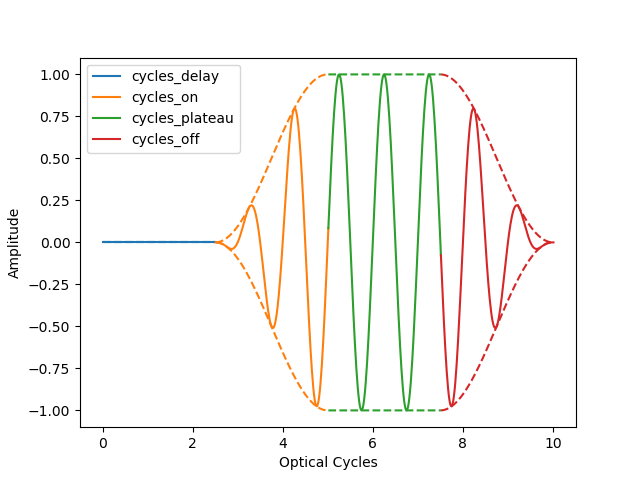
\includegraphics[width=0.7\textwidth]{Pulse.png}
\caption{A graphical depiction of the various laser parameters described in Sec.~\ref{sub:parameters}. The dotted lines show the laser envelope and the solid lines are the vector potential. The various colors show what regions are effected by the various laser parameters. Depicted is a sin$^2$ pulse.}
\label{fig:pulse}
\end{figure}

The code itself supports slightly more general pulse shapes than the standard sine squared or Gaussian pulse. The code allows for the pulse to be delayed before starting using the cycles\_delay parameter, ramped on for a period of time using the cycles\_on parameter, then held at its max intensity for using cycles\_plateau, and ramped off using the cycles\_off parameter. See Fig.~\ref{fig:pulse} for a graphical representation of the parameters. This allows for the creation of most pulses. The code also supports multiple pulses that can be controlled independently of each other. The on and off ramps can either be a sin$^n$ or Gaussian shape. You can mixed powers of sine (\textbf{must be even}) in a single pulse, however, if Gaussian is chosen both ramps are Gaussian though they can have different widths. For the Gaussian pulses, the code propagates for 5 times the full width half max (FWHM) on the ramp on and off. This brings the Gaussian close to zero since a Gaussian is never truly zero. The amount of runtime for a Guassian pulse should be tested.

Using flat top pulses (cycles\_plateau $>$ 0) can clean up many results, however, they are extremely difficult to produce experimentally for pulses less than a picosecond and they should be used with care.

\subsubsection{Experiment type} % (fold)
\label{ssub:experiment_type}
TODO
\begin{itemize}
  \item ``default''
  \item ``File'' describe input file
  \item ``streaking'' 2 pulses, tau\_delay
\end{itemize}
% subsubsection experiment_type (end)

% subsection lasers (end)

% subsection potentials (end)

\section{Running Calculations} % (fold)
\label{sec:running_tdse_and_best_practices}
\subsection{Running the Code} % (fold)
\label{sub:running_the_code}
\subsubsection{Basic usage} % (fold)
\label{ssub:basic_usage}
Once the code has been properly built, a binary file ``\$\{TDSE\_ROOT\}/bin/TDSE'' should exist with \$\{TDSE\_ROOT\} as the path to the TDSE repository. You will need to define this variable yourself, or type the path out. To run the code, change directory (cd) to a directory with ``input.json'' file that contains the parameters for the simulation you wish to run. (see Sec.~\ref{sec:input} for details on the ``input.json'' file) Then execute the binary file. This can be done by just typing
\begin{verbatim}
${TDSE_ROOT}/bin/TDSE
\end{verbatim}
into the command line (replacing \$\{TDSE\_ROOT\}) and pressing enter.

An example output is on the following page (Sec~\ref{ssub:example_output}).
\newpage
\subsubsection{Example output}
\label{ssub:example_output}
Not all parts of the output will exist depending on the options you have chosen in the input file. If you have questions on what a particular line of the output means, please let me know.
\begin{verbatim}

******************* Setting up Simulation *******************

Simulation running on 1 Processors
Reading input file: input.json
Validating input
Input valid
Reading input complete
Creating pulses
Pulses created
Creating Wavefunction
Checkpointing Psi: 0
Wavefunction created
Creating Hamiltonian
Hamiltonian Created
Creating Simulation
Simulation Created

****************** Eigen State Calculation ******************


Calculating the lowest 1 eigenvectors using SLEPC
Eigen (-0.904578,-1.94079e-14) (0,0) 1
Checkpointing Wavefunction in He.h5:  0

************************ Propagation ************************


Propagating in time
Total writes: 2
Starting propagation
Checkpointing Psi: 1

Iteration: 2000
Pulse ends: 2940
Average time for time-step: 1.77576
Checkpointing Psi: 2
Checkpoint time: 0.199936
Checkpointing Psi: 3
Checkpointing Psi Projections: 1

Propagating until step: 2940
Checkpointing Psi: 4
Checkpointing Psi Projections: 2

******************** Simulation Complete ********************

Deleting Hamiltonian
Deleting Wavefunction
Deleting Pulse
\end{verbatim}
\newpage
% subsubsection basic_usage (end)

\subsubsection{Command line options} % (fold)
\label{ssub:command_line_options}
Here are a few command line options to make this codes log file a bit more useful. Running the code with command line options will look like
\begin{verbatim}
${TDSE_ROOT}/bin/TDSE -command_line_option_0 -command_line_option_1
\end{verbatim}

If you are using SLEPc I recommend adding
\begin{verbatim}
-eps_monitor
\end{verbatim}
to your command line. This will allow you to monitor the convergence of your eigen state calculations

For profiling the code use
\begin{verbatim}
-log_view
\end{verbatim}
This will provide a large amount of details relating to how the code preformed during a run. It is useful for estimating future job runtimes and profiling the overall code.

If you wish to change to propagation solver (default is GMRES) use
\begin{verbatim}
-prop_ksp_type ${KSP_TYPE}
\end{verbatim}
See PETSc's documentation for the available options. Use ``-log\_view'' to compare their runtime.

If you want to change the solver for the eigen state method (only for Power method) use
\begin{verbatim}
-eigen_ksp_type ${KSP_TYPE}
\end{verbatim}
A recommended setup if you keep getting divergence issues is
\begin{verbatim}
-eigen_ksp_type preonly -eigen_pc_type lu -eigen_pc_factor_mat_solver_package superlu_dist
\end{verbatim}
% subsubsection command_line_options (end)

\subsubsection{Parallel Execution} % (fold)
\label{ssub:parallel_execution}
This code scales well on modern HPC systems. You can run the code in parallel utilizing ``mpiexec'' or a similar command. The bash command to run the code will look like
\begin{verbatim}
mpiexec -n ${number_of_processors} {TDSE_ROOT}/bin/TDSE -command_line_options
\end{verbatim}
where \$\{number\_of\_processors\} is the number of processors you wish to run this code on. We have used upwards of 3,000 without issue. The number of processors being used is printed near the top of the output.
% subsubsection parallel_execution (end)

\subsubsection{Ground State Calculations} % (fold)
\label{ssub:ground_state_calculations}
If you wish to produce only ground states that can be read in to other calculations, set ``propagation'' to 0 (Sec~\ref{ssub:propagate}) and ``state\_solver'' to something other than ``File'' (Sec.~\ref{ssub:state_solver}). This will produce a ground state file once the calculation completes. This can be read in using the ``name'' parameter (Sec~\ref{ssub:target_name}). By setting the full path in name (leaving off the .h5), many calculations can read the same file. This saves storage space and computational time.
% subsubsection ground_state_calculations (end)

\subsubsection{Time Propagation} % (fold)
\label{ssub:time_propagation}
To propagate in the laser field, set ``propagation'' to 1 (Sec~\ref{ssub:propagate}) and ensure your laser (Sec~\ref{ssub:laser_parameter}) is set up correctly. It is also useful to set ``state\_solver'' to ``File'' (Sec.~\ref{ssub:state_solver}) if you have already calculated a set of ground states to avoid recalculating them.
% subsubsection time_propagation (end)

\subsubsection{Restart mode} % (fold)
\label{ssub:restart_mode}
This code provides the ability to restart a simulation that has timed out or crashed during laser propagation. To run a new simulation that starts at the beginning of the laser pulse set ``restart'' to 0 (Sec~\ref{ssub:restart}). If you wish to start from the last checkpoint in the TDSE.h5 file set ``restart'' to 1.
% subsubsection restart_mode (end)

\subsubsection{Daisey Chain Script} % (fold)
\label{ssub:daisey_chain_script}
TODO
% subsubsection daisey_chain_script (end)

\subsubsection{Visualization of Results} % (fold)
\label{ssub:visualization_of_results}
TODO
% subsubsection visualization_of_results (end)

\subsubsection{Create Observables file} % (fold)
\label{ssub:create_observables_file}
The output from this code is stored in very few HDF5 files. This keeps the run directory clean and avoids running into file count limits imposed at some super computing facilities. However, large files are hard to transfer, and often the wavefunctions are not needed to analyze the physics. To produce a smaller data file with many useful observables, go to the directory your simulation was run in. The execute the ``make\_obs.sh'' which can be found at ``\$\{TDSE\_ROOT\}/scripts/make\_obs.sh''. If the base script doesn't satisfy your needs, feel free to edit away.
% subsubsection create_observables_file (end)

% subsection running_the_code (end)

\subsection{TDSE Best Practices} % (fold)
\label{sub:tdse_best_practices}

\subsubsection{Sharing Ground State files} % (fold)
\label{ssub:sharing_ground_state_files}
TODO
% subsubsection sharing_ground_state_files (end)

\subsubsection{Convergence Tests} % (fold)
\label{ssub:convergence_tests}
TODO
% subsection convergence_tests (end)

\subsubsection{Minimizing IO} % (fold)
\label{ssub:minimizing_io}
Writing wavefunctions and other large vectors to disk is a time consuming task (can take many minutes) and the data produced can add up quickly (I have seen upwards of a terrabyte for one simulation). Because of this, it is best to set ``write\_frequency\_checkpoint'' to a large number if the wavefunction itself is not needed. However, if the number is set to high, no checkpoints to restart will be available in case a computer crashes or a simulation times out. It is up to you to determining the best frequency on your particular situation, though 1-4 hours between checkpoints is a good starting value on modern super computers.
% subsubsection minimizing_io (end)

\subsubsection{Vector Potential vs Electric Field} % (fold)
\label{ssub:vector_potential_vs_electric_field}
TODO
% subsubsection vector_potential_vs_electric_field (end)

\subsubsection{Flat Top Pulse} % (fold)
\label{ssub:flat_top_pulse}
Utilizing flat top pulses (cycles\_plateau > 0) can make various observables cleaner. However, flat top pulses with durations less than a picosecond are difficult to create in experiment. As a result, there uses should be limited to understanding and highlighting physical phenomena.
% subsubsection flat_top_pulse (end)

\subsubsection{Soft Core Potentials} % (fold)
\label{ssub:soft_core_potentials}
Soft cores are a common way of adjusting ground state energies to match experimental or theoretical values. They also remove the issues with the coulomb singularity. The impact of a soft core on the potential should be carefully considered before utilizing one.
% subsubsection soft_core_potentials (end)

\subsubsection{Extracting Photoelectron Spectra} % (fold)
\label{ssub:extracting_photoelectron_spectra}
TODO
% subsubsection extracting_photoelectron_spectra (end)

\subsubsection{High Harmonic Generation} % (fold)
\label{ssub:high_harmonic_generation}
TODO
% subsubsection high_harmonic_generation (end)

\subsubsection{Bound State Populations} % (fold)
\label{ssub:bound_state_populations}
TODO
% subsubsection bound_state_populations (end)

% subsection tdse_best_practices (end)
% section running_tdse_and_best_practices (end)

\section{Input} % (fold)
\label{sec:input}

For the code, the only thing that needs to be in the directory is the ``input.json'' file. This will describe the laser, atomic/molecular target, and various other things required for the code to run. This section will go through what each parameter means and a list of options for each parameter when applicable.

The input files are in the json format. This formate is standardized, however, missing or extra commas, brackets, braces, ect.\ can be tricky to track down if you are not familiar with the json format. Please take the time to learn json now. You will thank yourself later.

\textbf{Make sure to use ASCII characters, copy and paste could cause issues.}

\subsection{Example File} % (fold)
\label{sub:example_file}
The following is an input file for simulating an 8 cycle, 800nm, sine squared pulse incident on atomic Hydrogen. This will produce a well converged High Harmonic Spectrum, though it may take a few hours to run. For a faster simulation that will be close to right, you can increase ``delta\_x\_max'' and ``delta\_x\_min'' to a larger number (say 0.5). You will need to do this for both dimensions.

\textbf{Make sure to use ASCII characters, copy and paste could cause issues.}

(current versions of example files can be found in the ``example'' directory)
\begin{verbatim}
{
  "alpha": 0.0,
  "coordinate_system": "Spherical",
  "delta_t": 0.05,
  "dimensions": [
  {
      "delta_x_max": 0.1,
      "delta_x_max_start": 4.0,
      "delta_x_min": 0.1,
      "delta_x_min_end": 4.0,
      "dim_size": 100.0,
      "l_max": 30, 
      "m_max": 0
    }
  ],
  "ee_soft_core": 0.01,
  "field_max_states": 0,
  "free_propagate": 0,
  "gauge": "Length",
  "gobbler": 0.9,
  "laser": {
    "experiment_type": "default",
    "frequency_shift": 1,
    "pulses": [
      {
        "cep": 0.0,
        "cycles_delay": 0.0,
        "cycles_off": 4.0,
        "cycles_on": 4.0,
        "cycles_plateau": 0.0,
        "ellipticity": 0.0,
        "energy": 0.057,
        "gaussian_length": 5.0,
        "helicity": "left",
        "intensity": 1e14,
        "polarization_vector": [0.0, 1.0, 0.0],
        "power_off": 2.0,
        "power_on": 2.0,
        "poynting_vector": [0.0, 0.0, 1.0],
        "pulse_shape": "sin"
      }
    ]
  },
  "num_electrons": 1,
  "order": 4,
  "propagate": 1,
  "restart": 0,
  "sigma": 3.0,
  "start_state": {
    "amplitude": [0.5, 0.5], 
    "l_index": [0, 1], 
    "m_index": [0, 0], 
    "n_index": [1, 2], 
    "phase": [0.0, 0.0]
  },
  "state_solver": "SLEPC",
  "states": 5,
  "target": {
    "name": "H",
    "nuclei": [
      {
       "exponential_r_0": [0.0],
       "exponential_amplitude": [0.0],
       "exponential_decay_rate": [0.0],
       "gaussian_r_0": [0.0],
       "gaussian_amplitude": [0.0],
       "gaussian_decay_rate": [0.0],
       "location": [0.0, 0.0, 0.0],
       "square_well_r_0": [0.0],
       "square_well_amplitude": [0.0],
       "square_well_width": [0.0],
       "yukawa_r_0": [0.0],
       "yukawa_amplitude": [0.0],
       "yukawa_decay_rate": [0.0],
       "z": 1.0
      }
    ]
  },
  "tol": 1e-10,
  "write_frequency_checkpoint": 1000,
  "write_frequency_eigin_state": 1000,
  "write_frequency_observables": 1
}
\end{verbatim}
% subsection example_file (end)

\subsection{Coordinate Systems} % (fold)
\label{sub:coordinate_systems}
How long the calculation will take is largely dependent on the coordinate system you choose. If possible, I recommend utilizing the spherical coordinate system when possible. It is the most limited as far as targets (currently only supports spherically symmetric), but its runtime is orders of magnitude faster. Cylindrical is the second fastest and supports cylindrically symmetric potentials with lasers aligned along the z axis. The Cartesian code is more general, but much slower.

\subsubsection{Hyperspherical} % (fold)
\label{ssub:Hyperspherical}
\textbf{TODO}
\begin{verbatim}
"dimensions": [{
      "delta_x_max": 0.1,
      "delta_x_max_start": 4.0,
      "delta_x_min": 0.1,
      "delta_x_min_end": 4.0,
      "dim_size": 100.0,
      "k_max": 10, 
      "l_max": 10, 
      "m_max": 0
}],

"start_state": {
    TODO
},
\end{verbatim}

\subsubsection{Spherical} % (fold)
\label{ssub:spherical}
\textbf{TODO}
\begin{verbatim}
"dimensions": [{
      "delta_x_max": 0.1,
      "delta_x_max_start": 4.0,
      "delta_x_min": 0.1,
      "delta_x_min_end": 4.0,
      "dim_size": 100.0,
      "l_max": 10, 
      "m_max": 0
}],

"start_state": {
    "amplitude": [0.5, 0.5], 
    "l_index": [0, 1], 
    "m_index": [0, 1], 
    "n_index": [1, 2], 
    "phase": [0.0, 0.0]
},
\end{verbatim}
% subsubsection spherical (end)

\subsubsection{Cartesian and Cylindrical} % (fold)
\label{ssub:cartesian_and_cylindrical}
\textbf{TODO}
\begin{verbatim}
"dimensions": [{
      "delta_x_max": 0.1,
      "delta_x_max_start": 4.0,
      "delta_x_min": 0.1,
      "delta_x_min_end": 4.0,
      "dim_size": 100.0
},
{
      "delta_x_max": 0.1,
      "delta_x_max_start": 4.0,
      "delta_x_min": 0.1,
      "delta_x_min_end": 4.0,
      "dim_size": 100.0
}],

"start_state": {
    "amplitude": [0.5, 0.5], 
    "index": [0, 1],  
    "phase": [0.0, 0.0]
}
\end{verbatim}
% subsubsection cartesian_and_cylindrical (end)

% subsection coordinate_system_quirks (end)

\subsection{Parameters} % (fold)
\label{sub:parameters_input}
The following is my attempt as describing what each parameter does. Each parameter is a subsubsection and they should come in the order of the example input file in Sec~\ref{sub:example_file}. Sub section names for nested parameters include a ``-'' to show that the parameter is either part of a list or dictionary of a different parameter. This is shown in Sec~\ref{ssub:dimensions-dim_size} as ``dim\_size'' is a sub parameter of the ``dimensions'' parameter.  Some of the parameters have extra descriptions that are critical to reproduce results from other codes. This may lead to some lengthy discussion that may not be useful for all users. If you have questions on particular parameters or more general questions, let me know.

\textbf{Make sure to use ASCII characters, copy and paste could cause issues.}

\subsubsection{alpha}
alpha is the soft core parameter described in Sec~\ref{ssub:soft_core_like} used in nuclear interactions. A floating point number can be input, and a value of 0.0 leads to the standard Euclidean distance $r=\sqrt{x^2+y^2+\cdots}$. It is used in the Coulomb (Hydrogen like) potentials. It is also used for any $r$ that comes in the denominator of the Single Active Electron (SAE) Potentials in Sec~\ref{ssub:single_active_electron}. Any $r$ that comes in the numerator is the standard Euclidean distance. The soft core takes the mathematical form of
\begin{equation}
  r_{soft} = \sqrt{r^2 + \alpha^2}
\end{equation}
where $r$ is the standard Euclidean distance.

\subsubsection{coordinate\_system}
This describes the available coordinate systems available. Current list of available coordinate systems is (make sure to use ASCII quotes, don't just copy and paste)
\begin{itemize}
  \item ``Hyperspherical'' (for 2 electron calculations)
  \item ``Spherical'' (Recommended)
  \item ``Cartesian''
  \item ``Cylindrical''
  \item ``RBF'' (beta)
\end{itemize}
The ``Cartesian'' coordinate system supports 1-3 dimensions with up to 2 electrons with any laser polarization that can be described in that number of dimensions. Though 2 electron calculations are computationally limiting. ``Cylindrical'' is a discretization in cylindrical coordinates for linear polarization on atoms or aligned linear molecules. It is 2 dimensional ($\rho$ and $z$) and runs much faster than a 3D simulation would. The ``RBF'' code is very much in beta testing and requires and external package. Only those wishing to get their hands dirty developing the method further should use this code. Talk to me if this is you.

\subsubsection{delta\_t}
delta\_t is the time step used in the simulation in atomic units (floating point number). Time steps in the range of 0.05 to 0.1 are typically sufficient for a simulation, however, one must run a convergence test non the particular observable you're interested in.

\subsubsection{dimensions}
\label{ssub:dimensions}
dimensions is a list of json objects (also known as dictionaries). Each dictionary provides the size of a new dimension. In the Cartesian coordinate system, the dimensions are added in the order x, y, z. If only 2 dictionaries are included, a 2D simulation is preformed. For Cylindrical coordinates the dimensions are added in the order $\rho$ and $z$.

\textbf{Note}: Each dimension can have a minimum grid spacing and a maximum grid spacing with a sine squared ramp connecting them. This appears to work for ground state calculations, however, time propagation can have issues. Take extra care if you wish to use this feature. If ``delta\_x\_min'' $=$ ``delta\_x\_max'', the code has been well tested and will produce good results (you just have to get past the error checks by moving ``delta\_x\_max\_start'' and ``delta\_x\_min\_end'' away from the boundaries of your grid).

\subsubsection{dimensions - delta\_x\_max}
delta\_x\_max is the max grid spacing in atomic units (outside edge of the grid). This is useful to describe highly excited states and outgoing wave packets, though it is not 100\% stable. Set equal to delta\_x\_min to use the well tested code. Typical values for converged calculations on a uniform grid are less than or equal to 0.1. See the note in Sec~\ref{ssub:dimensions} for more details on nonuniform grid.

\subsubsection{dimensions - delta\_x\_max\_start}
delta\_x\_max\_start is the distance from the origin that the delta\_x\_max is used to increase the grid size. See the note in Sec~\ref{ssub:dimensions} for more details on nonuniform grid.

\subsubsection{dimensions - delta\_x\_min}
delta\_x\_min is the min grid spacing in atomic units (outside edge of the grid). This is useful to describe highly excited states and outgoing wave packets, though it is not 100\% stable. Set equal to delta\_x\_max to use the well tested code. Typical values for converged calculations on a uniform grid are less than or equal to 0.1. See the note in Sec~\ref{ssub:dimensions} for more details on nonuniform grid.

\subsubsection{dimensions - delta\_x\_min\_end}
delta\_x\_min\_end is the distance from the origin that the sine squared ramp up between delta\_x\_min and delta\_x\_max begins. See the note in Sec~\ref{ssub:dimensions} for more details on nonuniform grid.

\subsubsection{dimensions - dim\_size}
\label{ssub:dimensions-dim_size}
dim\_size is the total size of the dimension in atomic units. For all Cartesian and the $z$ axis in Cylindrical, the grid will go from -dim\_size/2 to dim\_size/2. For the $\rho$ dimension in Cylindrical, the grid will go from 0 to dim\_size.

\subsubsection{dimensions - l\_max}
\label{ssub:dimensions-l_max}
l\_max is the maximum angular momentum quantum number used by the spherical harmonic expansion. For few photon ionizations at reasonable intensities, values of 5-20 are typical. For HHG spectra from 30 to 100+ are used depending on the desired accuracy.

\subsubsection{dimensions - m\_max}
\label{ssub:dimensions-m_max}
m\_max is the maximum angular momentum projection quantum number used by the spherical harmonic expansion. For linear polarized lasers along the z axis (assuming the ground state is m=0) you can set m\_max=0 due to selection rules ($l\rightarrow l\pm1$ and $m\rightarrow m$). For any other laser polarization or initial conditions with m$\ne$0 you will need to set m\_max$>$0 and typically equal to l\_max. 

\subsubsection{field\_max\_states}
\label{ssub:field_max_states}
field\_max\_states allows for the peak of the electric field or vector potential to be used for eigenstate calculations. Utilizing this parameter is still in beta. Testing is required if this parameter is not set to 0. The following values can be set
\begin{itemize}
  \item ``0'' Field free (standard use case)
  \item ``1'' Field max (still in beta)
\end{itemize}

\subsubsection{ee\_soft\_core}
ee\_soft\_core is the soft core parameter described in Sec~\ref{ssub:soft_core_like} used in the electron-electron repulsion term.

\subsubsection{free\_propagate}
free\_propagate is the number of time steps the wavefunction is propagated after the last laser ``finishes'' (integer). Total free propagation is delta\_t * free\_propagate in atomic units.

\subsubsection{gauge}
gauge allows for calculation to be done in Velocity and Length gauge and runtime differences are negligible in the cases I've tested. Both should produce the same answer when fully converged. The options are
\begin{itemize}
  \item ``Velocity''
  \item ``Length''
\end{itemize}

\subsubsection{gobbler}
This sets the size of the exterior complex scaling (ECS) potential (Sec~\ref{ssub:exterer_complex_scaling}) which absorbs outgoing wavepackets. A value of 0.9 means that 90\% of the grid is normal and the outer 5\% on each side contains an ECS potential.

\subsubsection{laser}
\label{ssub:laser_parameter}
The laser parameter is a dictionary that contains the particular laser being used in the calculation.

\subsubsection{laser - experiment\_type}
The experiment\_type is how the laser is being used. The options are
\begin{itemize}
  \item ``default''
  \item ``File''
  \item ``streaking''
\end{itemize}
Below is documentation for ``default''. Details on the others can be found in Sec~\ref{ssub:experiment_type}.

\subsubsection{laser - frequency\_shift}
\label{ssub:laser_parameter-frequency_shift}
The frequency\_shift parameter corrects for the error when setting the central frequency of the A field rather than the E field (see Sec.~\ref{sub:lasers}). It only supports some lasers, but this could be fixed using numeric integrals. Let me know if you want to code this up. Otherwise it can be done manually.
\begin{itemize}
  \item frequency\_shift = 1. accounts for the shift (setting E field central frequency, preferred)
  \item frequency\_shift = 0. central frequency is unchanged (setting A field central frequency for manual entry)
\end{itemize}

\subsubsection{laser - pulses}
pulses is a list of dictionaries used to describe a pulse. Each component inside a single pulse is in the units of that pulse such as the length of a single cycle is based on the frequency of that particular pulse.

\subsubsection{laser - pulses - cep}
cep is the carrier envelope phase (CEP) which is $\phi_A$ in Eq.~\ref{eq:afield}. It is in units of 2$\pi$, so a value of 0.5 gives $\phi_A=\pi$. The CEP is defined off of $t_0$ which is defined at the end of cycles\_on (peak of laser field/beginning of the plateau).

\subsubsection{laser - pulses - cycles\_delay}
cycles\_delay is the number of cycles until the ramp up of the pulse begins. See Fig.~\ref{fig:pulse} for a graphical representation.

\subsubsection{laser - pulses - cycles\_off}
cycles\_off is the number of cycles that ramps the pulse back to zero. See Fig.~\ref{fig:pulse} for a graphical representation. Note that this is the full size for ``sin'' envelopes and the FWHM for ``Gaussian''. The ``Gaussian'' shapes are propagated for 5 times the cycles\_on to allow for the envelope to approach zero.

\subsubsection{laser - pulses - cycles\_on}
cycles\_on is the number of cycles that ramps the pulse from zero to its max value. See Fig.~\ref{fig:pulse} for a graphical representation. Note that this is the full size for ``sin'' envelopes and the FWHM for ``Gaussian''. The ``Gaussian'' shapes are propagated for 5 times the cycles\_on to allow for the envelope to approach zero.

\subsubsection{laser - pulses - cycles\_plateau}
cycles\_plateau is the number of cycles the pulse remains at its max value. See Fig.~\ref{fig:pulse} for a graphical representation.

Using flat top pulses (cycles\_plateau $>$ 0) can clean up many results, however, they are extremely difficult to produce experimentally for pulses less than a picosecond. Due to this, reviewers may have issues with these pulses. Just something to be aware of.

\subsubsection{laser - pulses - ellipticity}
ellipticity is the ratio of the minor over major axis for the laser polarization. 0.0 gives linear polarization and 1.0 gives circular polarization.

\subsubsection{laser - pulses - energy}
energy provides the central frequency ($\omega_A$) in Eq.~\ref{eq:afield}. Given in atomic units (800nm $\approx$ 0.057a.u.). Note that the frequency shift (Eq.~\ref{eq:fshift}) described in Sec~\ref{sub:lasers}should be accounted for when pulses are around 15 optical cycles or less.

\subsubsection{laser - pulses - gaussian\_length}
gaussian\_length is the number of times the FWHM a gaussian pulse is propagated for. The parameters cycles\_on and cycles\_off control the half width half max on the rising and falling parts of the pulse. This controls how close to zero the envelope gets to zero. For non gaussian pulse shapes, this is not read and set to one in the code. A good value appears to be 5.0 though feel free to test this out.

\subsubsection{laser - pulses - helicity}
helicity is the handedness of elliptical and circular polarized lasers. It take the values of:
\begin{itemize}
  \item ``left''
  \item ``right''
\end{itemize}

\subsubsection{laser - pulses - intensity}
intensity is the peak intensity of the laser field. It is given in W/cm$^2$. Typical values are $10^{12}$ to $10^{15}$. Easiest to provide in the from $2e12$ for $2*10^{12}$, though it can be written out with all the zeros if one wishes.

\subsubsection{laser - pulses - polarization\_vector}
polarization\_vector is a list that defines the direction of the major axis of the laser. It is normalized after being read in to avoid intensity scaling issues. The order of dimensions is the same as the coordinate system defined in Sec.~\ref{ssub:dimensions}.

\subsubsection{laser - pulses - power\_off}
power\_off is the power a ``sin'' envelope function is raised to on the ramp off portion of the pulse scaled by cycles\_off. The value must be an even power giving the envelope the form $\sin^{power\_off}$.

\subsubsection{laser - pulses - power\_on}
power\_on is the power a ``sin'' envelope function is raised to on the ramp on portion of the pulse scaled by cycles\_on. The value must be an even power giving the envelope the form $\sin^{power\_on}$.

\subsubsection{laser - pulses - poynting\_vector}
poynting\_vector defines the direction of propagation of the laser. When combined with the polarization\_vector and helicity, the coordinate system for the laser has been set. It is normalized after being read in to avoid intensity scaling issues. The order of dimensions is the same as the coordinate system defined in Sec.~\ref{ssub:dimensions}.

\subsubsection{laser - pulses - pulse\_shape}
pulse\_shape gives the ramp functions for the pulse. They are either sin$^n$ (where $n$ is set using power\_on and power\_off) or Gaussian. The values it takes are
\begin{itemize}
  \item ``sin''
  \item ``gaussian''
\end{itemize}

\subsubsection{num\_electrons}
num\_electrons is the number of electrons in the simulation. Having more than one electron should work but has not been throughly tested. Ask for 3 or more electrons for an easter egg.

\subsubsection{order}
order is the order of finite difference used. Only 2nd order appears to work, however, and even order seams to work for ground state calculations. I recommend just leaving it set to 2.

\subsubsection{propagate}
\label{ssub:propagate}
propagate controls if the wave function is propagated in the laser field. If set to 0, no propagation occurs. If set to 1, the wavefunction is propagated in the laser field.

\subsubsection{restart}
\label{ssub:restart}
restart allows the code to restart the propagation off the last checkpoint in the T. If set to 0, the code will start from the beginning of the pulse, and a fresh TDSE.h5 file will be produced. If set to 1, the code will restart off the last checkpoint in the TDSE.h5 file.

\subsubsection{sigma}
sigma is the size of the Gaussian wavefunction used as an initial guess for the Power method. A value of 3.0 works well for all cases I have run across, but it could be adjusted to make the convergence go faster. I would recommend switching to SLEPC if you want things to speed up.

\subsubsection{states}
states is the number of bound states of your potential you would like to calculate. It is also the number of states that are used to calculate populations in the code and projected out for removing the bound state population when calculating photoelectron spectra. This is a number, except when using the ``Power'' method as a state\_solver. Then is it a list of dictionaries with target energies provided. Here is an example:
\begin{verbatim}
"states": [{"energy": -0.5}, {"energy": -0.125}]
\end{verbatim}

\subsubsection{start\_state}
start\_state is a dictionary that defines the initial conditions for time propagation. The initial state $\Psi$ is given by
\begin{equation}
  \Psi = \sum\limits_n a_n e^{i\phi_n} \psi_n^{idx}
  \label{eq:start_state}
\end{equation}
$a_n$ is the amplitude, $psi_n$ is the bound state, $\phi_n$ is the phase, $n$ is the index into the ``amplitude'', ``index'', and ``phase'' arrays, and $idx$ is the index into the bound state data file given in the ``index'' array. The initial wavefunction is normalized to one after being read in, so the amplitude array's values are only relative amounts.

\subsubsection{start\_state - amplitude}
amplitude defines the $a_n$ in Eq.~\ref{eq:start_state} where $n$ is the index into this array. The initial wavefunction is normalized to one after being read in, so the amplitude array's values are only relative amounts.

\subsubsection{start\_state - index}
index is the $idx$ wavefunction in the bound state file being used. It takes the value of $idx$ in Eq.~\ref{eq:start_state} where $n$ is the index into this array. Note that the bound state file wavefunctions may have a random phase. \textbf{This is not used in spherical code.}

\subsubsection{start\_state - l\_index}
The l quantum number for the initial state \textbf{used in the spherical code}. It is a list in the same order as the amplitude.

\subsubsection{start\_state - m\_index}
The m quantum number for the initial state \textbf{used in the spherical code}. It is a list in the same order as the amplitude.

\subsubsection{start\_state - n\_index}
The n quantum number for the initial state \textbf{used in the spherical code}. It is a list in the same order as the amplitude. (note if the grid is to small to support that n quantum number you may get a ``continuum state'')

\subsubsection{start\_state - phase}
phase is the value of $\phi_n$ in Eq.~\ref{eq:start_state} where $n$ is the index into this array. Note that the bound state file wavefunctions may have a random phase. If relative phase is important to your system take extra care when setting this.

\subsubsection{state\_solver}
\label{ssub:state_solver}
state\_solver it the method used to calculate ground states. ``SLEPC'' or ``File'' are the recommended modes of operation. All of the options are
\begin{itemize}
  \item ``File''
  \item ``SLEPC''
  \item ``Power''
  \item ``ITP'' (deprecated)
\end{itemize}

``File'' will read from the file given in ``target - name'' with a ``.h5'' extension added to it. This allows for the same bound state file to be used by many calculations.

``SLEPC'' utilized the SLEPc library to calculate eigen states. It uses the default SLEPc solver (currently Krylov Schur) though this can be changed by added the command line argument ``-eps\_type $<$method$>$'' when running the code. See the SLEPc for more information on how to do this.

``Power'' is the inverse shifted power method with target energies given by the ``states'' parameter. See ``states'' for an example on how to provide target energy values.

``ITP'' is imaginary time propagation. This is no longer supported as much better methods have been implemented, though it does lead to an easter egg.

\subsubsection{target}
target is how you define the potential (or target) in which you want to calculate bound states of or shine a laser on.

\subsubsection{target - name}
\label{ssub:target_name}
name is the name of the bound state file. It can also be used to provide a path to place/read from the file in a different folder. You should avoid spaces and punctuation in file names (follow good file naming practices). Note that the ``.h5'' is added inside the code, so it should not appear in this name.

\subsubsection{target - nuclei}
nuclei is a list that allows for nuclei to be placed at various places in space. Each can be coulomb or SAE (this may change later).

\subsubsection{target - nuclei - exponential\_r\_0}
exponential\_r\_0 is the donut radius for an exponential potential. This is the value of $r_{0,i}$ in Eq.~\ref{eq:exponential} with $i$ being the index into the array. Set to zero for atomic like behavior. See Sec~\ref{ssub:exponential_potentials} for exact form of the potential.

\subsubsection{target - nuclei - exponential\_amplitude}
exponential\_amplitude is the amplitude for an exponential potential. This is the value of $a_i$ in Eq.~\ref{eq:exponential} with $i$ being the index into the array. If set to 0 the potential has no effect. See Sec~\ref{ssub:exponential_potentials} for exact form of the potential.

\subsubsection{target - nuclei - exponential\_decay\_rate}
exponential\_decay\_rate is the decay rate for an exponential potential. This is the value of $c_i$ in Eq.~\ref{eq:exponential} with $i$ being the index into the array. See Sec~\ref{ssub:exponential_potentials} for exact form of the potential.

\subsubsection{target - nuclei - gaussian\_r\_0}
gaussian\_r\_0 is the donut radius for a Gaussian potential. This is the value of $r_{0,i}$ in Eq.~\ref{eq:gaussian} with $i$ being the index into the array. Set to zero for atomic like behavior. See Sec~\ref{ssub:gaussian_potentials} for exact form of the potential.

\subsubsection{target - nuclei - gaussian\_amplitude}
gaussian\_amplitude is the amplitude for a Gaussian potential. This is the value of $a_i$ in Eq.~\ref{eq:gaussian} with $i$ being the index into the array. If set to 0 the potential has no effect. See Sec~\ref{ssub:gaussian_potentials} for exact form of the potential.

\subsubsection{target - nuclei - gaussian\_decay\_rate}
gaussian\_decay\_rate is the decay rate for a Gaussian potential. This is the value of $c_i$ in Eq.~\ref{eq:gaussian} with $i$ being the index into the array. See Sec~\ref{ssub:gaussian_potentials} for exact form of the potential.

\subsubsection{target - nuclei - location}
location is a list that corresponds to the nuclei center. The distances $r$ and $r_{soft}$ are calculated from it. The order of dimensions is the same as the coordinate system defined in Sec.~\ref{ssub:dimensions}.

\subsubsection{target - nuclei - square\_well\_r\_0}
square\_well\_r\_0 is the donut radius for a square well potential. This is the value of $r_{0,i}$ in Eq.~\ref{eq:square_well} with $i$ being the index into the array. Set to zero for atomic like behavior. See Sec~\ref{ssub:square_well_potentials} for exact form of the potential.

\subsubsection{target - nuclei - square\_well\_amplitude}
square\_well\_amplitude is the amplitude or depth of a square well potential. This is the value of $a_i$ in Eq.~\ref{eq:square_well} with $i$ being the index into the array. If set to 0 the potential has no effect. See Sec~\ref{ssub:square_well_potentials} for exact form of the potential.

\subsubsection{target - nuclei - square\_well\_width}
square\_well\_width is the width of the square well potential. This is the value of $\Delta_i$ in Eq.~\ref{eq:square_well} with $i$ being the index into the array. See Sec~\ref{ssub:square_well_potentials} for exact form of the potential.

\subsubsection{target - nuclei - yukawa\_r\_0}
yukawa\_r\_0 is the donut radius for a Yukawa potential. This is the value of $r_{0,i}$ in Eq.~\ref{eq:yukawa} with $i$ being the index into the array. Set to zero for atomic like behavior. See Sec~\ref{ssub:yukawa_potentials} for exact form of the potential.

\subsubsection{target - nuclei - yukawa\_amplitude}
yukawa\_amplitude is the amplitude for a Yukawa potential. This is the value of $a_i$ in Eq.~\ref{eq:yukawa} with $i$ being the index into the array. If set to 0 the potential has no effect. See Sec~\ref{ssub:yukawa_potentials} for exact form of the potential.

\subsubsection{target - nuclei - yukawa\_decay\_rate}
yukawa\_decay\_rate is the decay rate for a Yukawa potential. This is the value of $c_i$ in Eq.~\ref{eq:yukawa} with $i$ being the index into the array. See Sec~\ref{ssub:yukawa_potentials} for exact form of the potential.

\subsubsection{target - nuclei - z}
z is the value of z in a coulomb like potential (Eq.~\ref{eq:H_like}). If set to 0 the potential has no effect. See Sec~\ref{ssub:hydrogen_like} for exact form of the potential.

\subsubsection{tol}
tol is used whenever a convergence tolerance is needed in the code. The only place I remember is for the eigen state calculations. A value of $1e-10$ is a good starting point.

\subsubsection{write\_frequency\_checkpoint}
write\_frequency\_checkpoint is the number of time steps between writing checkpoint files that allow the code to restart. Setting this to small can lead to massive data files. If it is to large, the code may crash before a checkpoint is written to disk. Typically you want a restart file written ever 20mins to a few hours of runtime depending on the size of the simulation. If you would like to make a video of the simulation, this can be set to a small value assuming you have the disk space.

\subsubsection{write\_frequency\_eigin\_state}
write\_frequency\_eigin\_state is the number of iterations between making convergence/writing to standard out checks when using the power method. Add ``-eps\_monitor'' to the run line in the bash script to monitor SLEPC calculations.

\subsubsection{write\_frequency\_observables}
write\_frequency\_observables is the number of time steps between writing calculating observables such as dipole, dipole acceleration, norm, ecs population, ect. I recommend leaving this set to 1 as it is not that time consuming in the current version of the code.
% subsection parameters(end)

% section input (end)

\section{Output} % (fold)
\label{sec:output}
The output of the code is done using the HDF5 library. To look at a file, you can use the command line option ``h5dump'' and ``h5ls''. Here are a few examples. Each data file contains a set a variables and a description of what each variable does. To see the datasets in a particular file use the `h5ls' command in the terminal. Replace H2.h5 with the file you which to look at.
\begin{verbatim}
$ h5ls -r H2.h5
/                        Group
/Energy                  Dataset {1/Inf}
/psi                     Dataset {1/Inf, 45000, 2}
\end{verbatim}

You can view what a description of what each data file has using ``-A'' with the ``h5dump'' command. The result result can be very long, so using it in conjunction with ``-d dataset'' will provide the description for a particular dataset. Here is an example for looking at the energy part of last set.
\begin{verbatim}
$ h5dump -A -d Energy H2.h5
HDF5 "H2.h5" {
DATASET "Energy" {
   DATATYPE  H5T_IEEE_F64LE
   DATASPACE  SIMPLE { ( 1 ) / ( H5S_UNLIMITED ) }
   ATTRIBUTE "Attribute" {
      DATATYPE  H5T_STRING {
         STRSIZE H5T_VARIABLE;
         STRPAD H5T_STR_NULLTERM;
         CSET H5T_CSET_ASCII;
         CTYPE H5T_C_S1;
      }
      DATASPACE  SCALAR
      DATA {
      (0): "Energy of the corresponding state"
      }
   }
}
}
\end{verbatim}

To view the contents of the datafile in your command line remove the -A option. The output can become long for large objects like psi, however it is useful for getting small datasets like the Energy of a bound state.
\begin{verbatim}
$ h5dump -d Energy H2.h5
HDF5 "H2.h5" {
DATASET "Energy" {
   DATATYPE  H5T_IEEE_F64LE
   DATASPACE  SIMPLE { ( 1 ) / ( H5S_UNLIMITED ) }
   DATA {
   (0): -0.9477
   }
   ATTRIBUTE "Attribute" {
      DATATYPE  H5T_STRING {
         STRSIZE H5T_VARIABLE;
         STRPAD H5T_STR_NULLTERM;
         CSET H5T_CSET_ASCII;
         CTYPE H5T_C_S1;
      }
      DATASPACE  SCALAR
      DATA {
      (0): "Energy of the corresponding state"
      }
   }
}
}
\end{verbatim}

\subsection{Complex numbers} % (fold)
\label{sub:complex_numbers}
For any dataset that is a complex number, the last dimension of the HDF5 data set is size 2. The first value (0th index) is the real part and the second value (1st index) is the imaginary part.
% subsection complex_numbers (end)

\subsection{TDSE.h5} % (fold)
\label{sub:tdse_h5}
The TDSE.h5 file contains most of the data from a simulation. This file can get large, so see Sec.~\ref{sub:observables_h5} on how to produce smaller data files to scp your data. The /Observables/ group contains time depended expectation values that are taken during the pulse. The /Parameters/ group contains the parameters used in the simulation. The /Projections/ group contains the wavefunction with bound states remove. The /Wavefunction/ group contains the wavefunction printed at various points in time.

\subsubsection{Observables} % (fold)
\label{ssub:observables}
The dipole acceleration is $\expval{\frac{x_i}{r^3}}{\Psi_i}$. This needs to be updated for targets that are not hydrogen. The end of the dipole acceleration has two indices and will look like ``/Observables/dipole\_acceleration\_(index i)\_(index j)''. Index i is the index of the electron starting from 0 and index j is the index of the dimension giving index 0,1,2 corresponding to coordinates x,y,z respectively ($\rho$,z for cylindrical).

The position expectation value is $\expval{x_i}{\Psi_i}$ with the same indexing as the dipole acceleration.

The norm is $\bra{\Psi}\ket{\Psi}$.

The gobbler is population in the ECS.

The time is the time at which each expectation value is taken.
% subsubsection observables (end)

\subsubsection{Parameters} % (fold)
\label{ssub:parameters}
The parameters are described in the input file section. Use ``h5ls -r TDSE.h5'' to get the list of simulations parameters.
% subsubsection parameters (end)

\subsubsection{Projections} % (fold)
\label{ssub:projections}
This is the wavefunction with the bound states projected out. It can be used to create a photo electron spectrum when few bound states are populated during the simulation. This method is still under development and should be used with care.
% subsubsection projections (end)
% subsection tdse_h5 (end)

\subsection{Pulse.h5} % (fold)
\label{sub:pulse_h5}
The pulses file contains the the pulse used in the simulation. The pulsed take the shape $f(t)sin(wt+phi)$. The supported pulse shapes can be found in Sec.~\ref{sub:lasers} and the parameters used to define various pulses are in Sec.~\ref{sec:input}.

The pulse\_envelope\_0 is the value of $f(t)$ in the pulse shape definition. The index 0 corresponds to the order the pulse was defined in the `input.json' file starting at 0.

The Pulse\_value\_0\_1 is the value of $f(t)sin(wt+phi)$ in a particular dimension. The index 0 corresponds to the order the pulse was defined in the `input.json' file starting at 0, and the index 1 corresponds to the dimension of the pulse with 0, 1, 2 relating to x, y, z respectively. For cylindrical coordinates the dimension order is $\rho$, z instead.
% subsection pulse_h5 (end)

\subsection{Target.h5} % (fold)
\label{sub:target_h5}
The target.h5 file (the name is read from the input file, so it maybe H.h5, He.h5, or something else) contains the field free or field max (Sec.~\ref{ssub:field_max_states}) states and associated eigen values. The ``Energy'' dataset contains the energy of the field free or field max states found is the ``psi'' dataset. The ``psi'' dataset contains the wave function of the bound states. The first index is which state you wish to use typically starting from the 1s state. The second index is the grid point on the wavefunction. Note that this is a 1D version of the full array. You will need to reshape the array to the correct dimension using the num\_x array found in the TDSE.h5 file under ``/Wavefunction/num\_x''. The last dimension is handles the complex numbers with the 0th element as the real part and the 1st element as the imaginary part.
% subsection target_h5 (end)

\subsection{Observables.h5} % (fold)
\label{sub:observables_h5}
The Observables.h5 file provides a file that contains most of the small datasets from the TDSE.h5 and Pulse.h5 files. It leaves out the wavefunctions to allow for data to be easily copied from remote machines with minimal download times. Since it is just a duplicate of various other files, the main code does not produce it. To make the Observables.h5 file execute the \$\{TDSE\_ROOT\}/scripts/make\_obs.sh file in the directory the simulation was run in. The script uses h5copy to move data around and can be edited to include exactly the data you need for a particular project.
% subsection observables_h5 (end)

% section output (end)

\section{Analysis} % (fold)
\label{sec:analysis}
TODO

% section analysis (end)


\section{Classes} % (fold)
\label{sec:classes}

The classes used in this code are written so they can be tested independently. Therefore, all classes that depend on other classes require those classes to be passed into the constructor. The developer is responsible to not delete these classes until other dependent classes are deleted.

For the most part, the classes do what you would expect. However, there are small deviations like the HDF5Wrappers writing the Parameters to the file rather than the other way around. This is done to enable restarts to not delete old datasets.

\subsection{PETSCWrapper} % (fold)
\label{sub:petscwrapper}
This class takes care of setting up SLEPC, PETSC, and MPI. It comes first so that the finalize calls are made once every other class has cleaned up after its self.
% subsection petscwrapper (end)

\subsection{ViewWrapper} % (fold)
\label{sub:viewwrapper}
This class wraps the HDF5 interface that PETSC supplies. It is used for dumping the wavefunctions to disk.
% subsection viewwrapper (end)

\subsection{Parameters} % (fold)
\label{sub:parameters}
This class holds the input file information and will be used by all other classes. It depends on a json parser (https://github.com/nlohmann/json) and reads inputs in json format. For more information about input parameter definitions and how they are used, see Section~\ref{sec:input}. This class is mainly used as a data structure. That being said, it does provided tools to validate various input parameters to limit user error. It is also used to convert the various laser input styles to the ``default'' style that the Pulse class needs to create the laser fields.

The code currently reads the input files from every processor in use. This hasn't been an issue running on upwards of 6,000 processors, but it should be changed at some point.

% subsection parameters (end)

\subsection{HDF5Wappers} % (fold)
\label{sub:hdf5wappers}
IO for this code is done using HDF5 files. HDF5 files provide the ability to utilize parallel file systems, generate self describing data files, and write compressed data. With these advantages, it becomes slightly more difficult to write data. To alleviate this issues, this class provides tools for writing to HDF5 files in a straight forward way.

Writing multidimensional arrays is difficult in HDF5. To avoid the added headache, one denominational arrays with the access pattern of
\begin{equation}
	array[x+y*nx] = array[x][y]
\end{equation}
and
\begin{equation}
	array[x+y*nx+z*nx*ny] = array[x][y][z]
\end{equation}
and so on. Note that the ordering flips when using python to visualize the data due to the c vs fortran ordering of arrays. Be sure to pay close attention to axis labels to make sure the data is orientated correctly.
% subsection hdf5wappers (end)

\subsection{Pulse} % (fold)
\label{sub:pulse}
Pulse handles creating and storing various parts of the pulse. Much of the functionality is private rather than public to prevent accessing data that is not allocated. Since storing each individual pulse is only useful until it is printed to a file, it is deallocated inside the constructor. The result is a much more efficient use of memory, and protection from accessing garbage arrays. See Section~\ref{sec:input} on how to define pulses.
% subsection pulse (end)

\subsection{Hamiltonian} % (fold)
\label{sub:hamiltonian}
We are interested in solving the Solving the Time-Dependent Sch\"{o}dinger Equation for atoms and molecules.
\begin{equation}
    i\frac{\partial}{\partial t}\psi(x,t) = \hat{H}\psi(x,t)
\end{equation}
Which leads to a Hamiltonian of
\begin{equation}
    \hat{H} = \sum_{e}\left(\frac{\hat{\mathbf{p}}^2_e}{2} - \frac{\mathbf{A}(t) \cdot \hat{\mathbf{p}}_e}{c} - \sum_{n} \frac{Z_n}{r_{e,n}}\right) + \sum_{e_1 < e_2}\frac{1}{r_{e_1, e_2}}
\end{equation}
The full problem is currently limited to 1 or 2 electrons. For a two electron atom (He like), we have the following Hamiltonian.
\begin{equation}
  \hat H = \frac{\hat{p_1}^2}{2} + \frac{\hat{p_2}^2}{2} - \frac{\vec{A} \cdot (\hat{p_1}+\hat{p_2})}{c} - \frac{Z}{x_1} - \frac{Z}{x_2} + \frac{1}{r_{12}}
\end{equation}

The Hamiltonian class takes the input file and defines the appropriate matrix to operate on our wave function.

% subsection hamiltonian (end)

\subsection{Simulation} % (fold)
\label{sub:simulation}
The simulation class implements various propagation and eigen state calculations. It then utilized every other class to provide the appropriate IO and behavior at various points in the simulation.
% subsection simulation (end)

% section classes (end)


\section{Testing} % (fold)
\label{sec:testing}
There is very little testing continued used in this code. The code is well tested when development occurs. If you would like to work on a unit test system or notices something is wrong. Please let me know.
% section testing (end)

\section{Wish list} % (fold)
\label{sec:wish_list}
\begin{itemize}
    \item Faster algorithm (radial code (done), non uniform grid, hyper-spherical harmonics, ect.)
    \item Free propagation support (Density Matrix for bound states)
    \item New features (two electron code)
    \item Moving nuclei (classical and/or quantum mechanical)
    \item Molecular expansions for spherical code
\end{itemize}
% section wish_list (end)

\section{Supporting works} % (fold)
\label{sec:supporting_works}

\subsection{Posters} % (fold)
\label{sub:posters}
DAMOP (18,19)
Gordan (18)
JILA ultrafast (18)
% subsection posters (end)
\subsection{Talks} % (fold)
\label{sub:talks}
DAMOP (18,19)
ISMS (19)
% subsection talks (end)
\subsection{Papers} % (fold)
\label{sub:papers}
J. Venzke, R. Reiff, Z. Xue, A. Jaroń-Becker, and A. Becker
PRA \textbf{98}, 043434 (2018).

\noindent
J. Venzke, T. Joyce, Z. Xue, A. Becker, and A. Jaron-Becker, 
PRA \textbf{98}, 063409 (2018). 
% subsection papers (end)
% section supporting_works (end)

\section{Contributors} % (fold)
\label{sec:contributors}
The following people have contributed to this code.
\begin{itemize}
  \item Goldsmith, Cory
  \item Venzke, Joel
\end{itemize}
% section contributors (end)
\end{document}